\documentclass[12pt]{article}

\usepackage[utf8]{inputenc}
\usepackage[T1]{fontenc}
\usepackage[spanish]{babel}
\usepackage{cmbright}
\usepackage{lmodern}
\usepackage{geometry}
\usepackage{tikz}
\usetikzlibrary{positioning,calc,math,arrows.meta,decorations.markings,intersections}
\usepackage{hyperref}
\usepackage[bf,sf,pagestyles]{titlesec}
\usepackage{titling}
\usepackage[runin]{abstract}
\usepackage[font={footnotesize, sf}, labelfont=bf]{caption} 
\usepackage{siunitx}
\usepackage{graphicx}
\usepackage{booktabs}
\usepackage{amsmath,amssymb}
\usepackage[spanish,sort]{cleveref}
\usepackage{enumitem}

\usepackage{biblatex}
\addbibresource{fonts.bib}

\geometry{
	a4paper,
	right = 2.5cm,
	left = 2.5cm,
	bottom = 3cm,
	top = 3cm
}

\newcommand{\sfbright}{\fontfamily{cmbr}\selectfont}
\renewcommand{\familydefault}{\rmdefault}
\renewcommand{\sfdefault}{cmbr}
\renewcommand{\arraystretch}{1.4}

\hypersetup{
	colorlinks,
	linkcolor = {red!50!blue},
	citecolor = {red!50!blue},
	linktoc = page
}

\numberwithin{table}{section}
\numberwithin{figure}{section}
\numberwithin{equation}{section}

\graphicspath{{./figs/}}

% Unitats
\sisetup{
	inter-unit-product = \ensuremath{ \, },
	allow-number-unit-breaks = true,
	math-celsius = {}^{\circ}\kern-\scriptspace C,
	detect-family = true,
	mode = text,
	list-final-separator = { y },
	list-pair-separator = { y },
	list-units = single,
	separate-uncertainty = true
}

\DeclareUnicodeCharacter{2212}{-}

\newcommand{\Z}{\mathbb{Z}}
\newcommand{\N}{\mathbb{N}}
\newcommand{\R}{\mathbb{R}}
\newcommand{\Ry}{\mathrm{Ry}}
\newcommand{\conv}[2]{\filldraw[fill = white!50!-red, fill opacity = 0.5, draw = -red!] (#1,0) ellipse [x radius = 0.1, y radius = #2];}
\newcommand{\data}[3]{\SI{#1 \pm #2}{#3}}
\newcommand{\unc}[2]{\ensuremath{{}\pm \SI{#1}{#2}}}
\DeclareMathOperator{\gr}{gr}
\newcommand{\abs}[1]{\left\lvert #1 \right\rvert}
\newcommand{\inn}[2]{\left\langle #1 , #2 \right\rangle}
\newcommand{\parbreak}{
	\begin{center}
		--- $\ast$ ---
	\end{center} 
}
\makeatletter
\newcommand*{\defeq}{\mathrel{\rlap{%
			\raisebox{0.3ex}{$\m@th\cdot$}}%
		\raisebox{-0.3ex}{$\m@th\cdot$}}%
	=
}
\makeatother

\newpagestyle{pagina}{
	\headrule
	\sethead*{\sffamily \bfseries Práctica 9}{}{\theauthor}
	\footrule
	\setfoot*{}{}{\sffamily \thepage}
}
\renewpagestyle{plain}{
	\footrule
	\setfoot*{}{}{\sffamily \thepage}
}
\pagestyle{pagina}

\title{\sffamily {\bfseries Práctica 9:} Red de difracción}
\author{\sffamily B2 2: Arnau Mas}
\date{\sffamily 14 de mayo de 2019}

\begin{document}
\maketitle
\renewcommand{\abstractname}{\sffamily \bfseries Resumen:}
\begin{abstract}
En esta práctica se ha estudiado el fenómeno de la difracción por red. Mediante la combinación del mismo y de la dispersión cromática, se puede separar el espectro de una fuente de luz, de manera similar al espectrómetro de prisma. Primeramente se ha calibrado la red midiendo un espectro conocido, el del mercurio, para determinar la separación entre rendijas. Hecho esto se han medido las líneas el espectro del hidrógeno correspondientes a la serie de Balmer y con ello se ha calculado un valor de la constante de Rydberg de \data{10.98}{0.22}{\micro m^{-1}} con tres cifras significativas correctas. 
\end{abstract}
\hrule

\section{Objetivos}
Los objetivos principales de esta práctica son el estudio del fenómeno de la difracción de Fraunhofer, el uso y calibración de una red de difracción y el cálculo de la constante de Rydberg a través de la medida de la serie de Balmer con la red de difracción.


\section{Introducción teórica}
Cuando una onda se propaga a través de un obstáculo tiene lugar el fenómeno de difracción debido a la interacción de los frentes de onda con el perfil del objeto. En función de la escala de distancias que consideramos hablamos de difracción de Fraunhofer o de Fresnel. En este caso predomina la difracción de Fraunhofer, pues la rendija a través de la cual se propaga la luz tiene una anchura mucho menor que la distancia que viaja la luz hasta llegar al punto donde hacemos la medición, \cite{hecht}. 

En el caso de una red de difracción, el obstáculo es una serie de rendijas paralelas separadas por una distancia fija \( a \). El patrón de interferencia consiste en un máximo central y una serie de máximos secundarios distribuidos simétricamente y de intensidad decreciente, tal y como se ve en la \cref{fig:patron}.

\begin{figure}[htb]
	\centering
	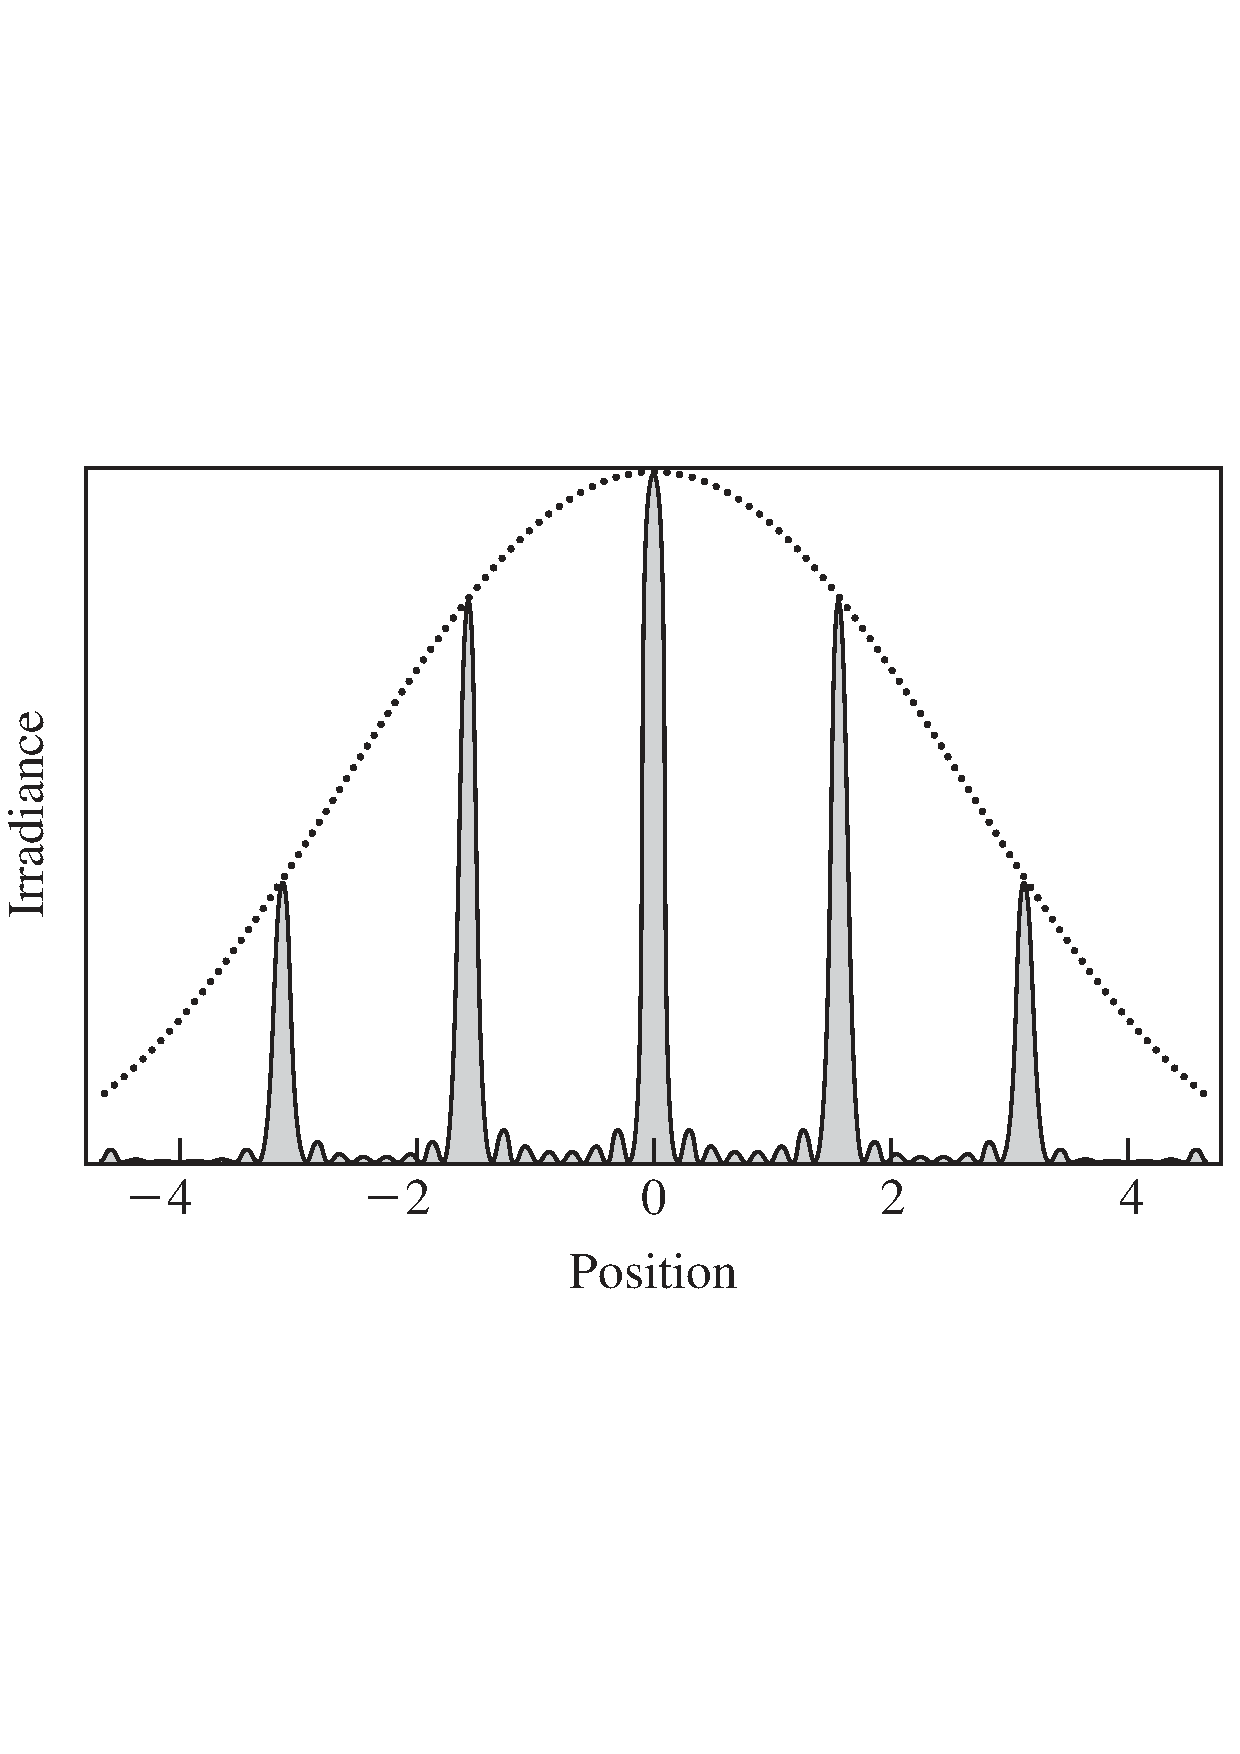
\includegraphics[scale = 0.3]{red.pdf}
	\caption{Patrón de difracción de una red de difracción con 8 rendijas}
	\label{fig:patron}
\end{figure}

La posición de los máximos depende únicamente de la separación entre las rendijas y de la longitud de onda incidente. Si imponemos la condición de interferencia constructiva encontramos que la posición del máximo de orden \( m \), \( \theta_m \), satisface
\begin{equation} \label{eqn:interferencia}
	a\sin{\theta_m} = m\lambda.
\end{equation}

Esto es suponiendo que el haz de luz incide perpendicularmente con la red de difracción. Si la luz incide a un ángulo \( \epsilon \) ---veánse las \cref{fig:normal,fig:no normal}--- entonces la condición de interferencia constructiva pasa a ser
\begin{equation} \label{eqn:interferencia1}
	a(\sin{\theta_m} - \sin{\epsilon}) = m\lambda.
\end{equation}

\begin{figure}[htb]
	\centering
	\begin{minipage}{0.45\textwidth}
		\centering
		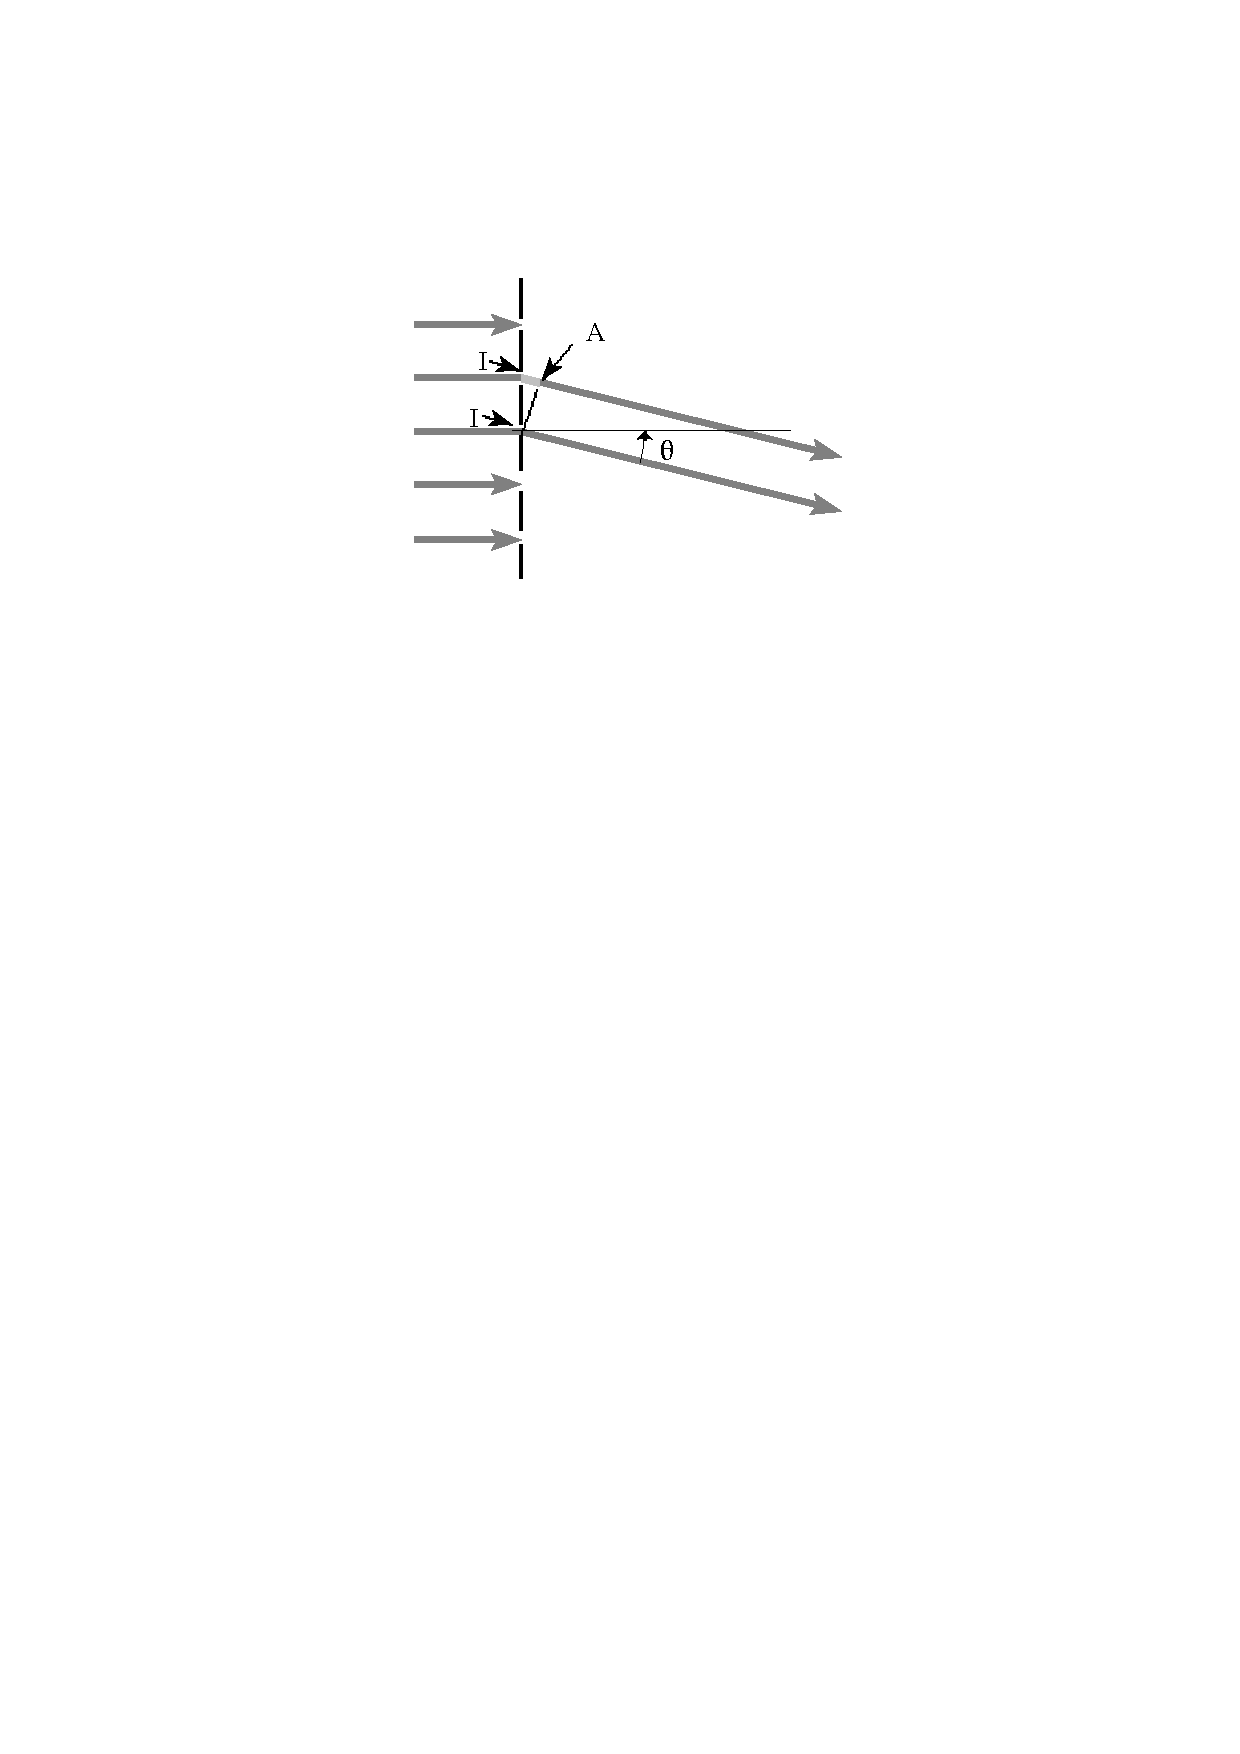
\includegraphics[scale = 0.7]{incidencia.pdf}
		\caption{Incidencia normal de la luz sobre la red}
		\label{fig:normal}
	\end{minipage}
	\hfill
	\begin{minipage}{0.45\textwidth}
		\centering
		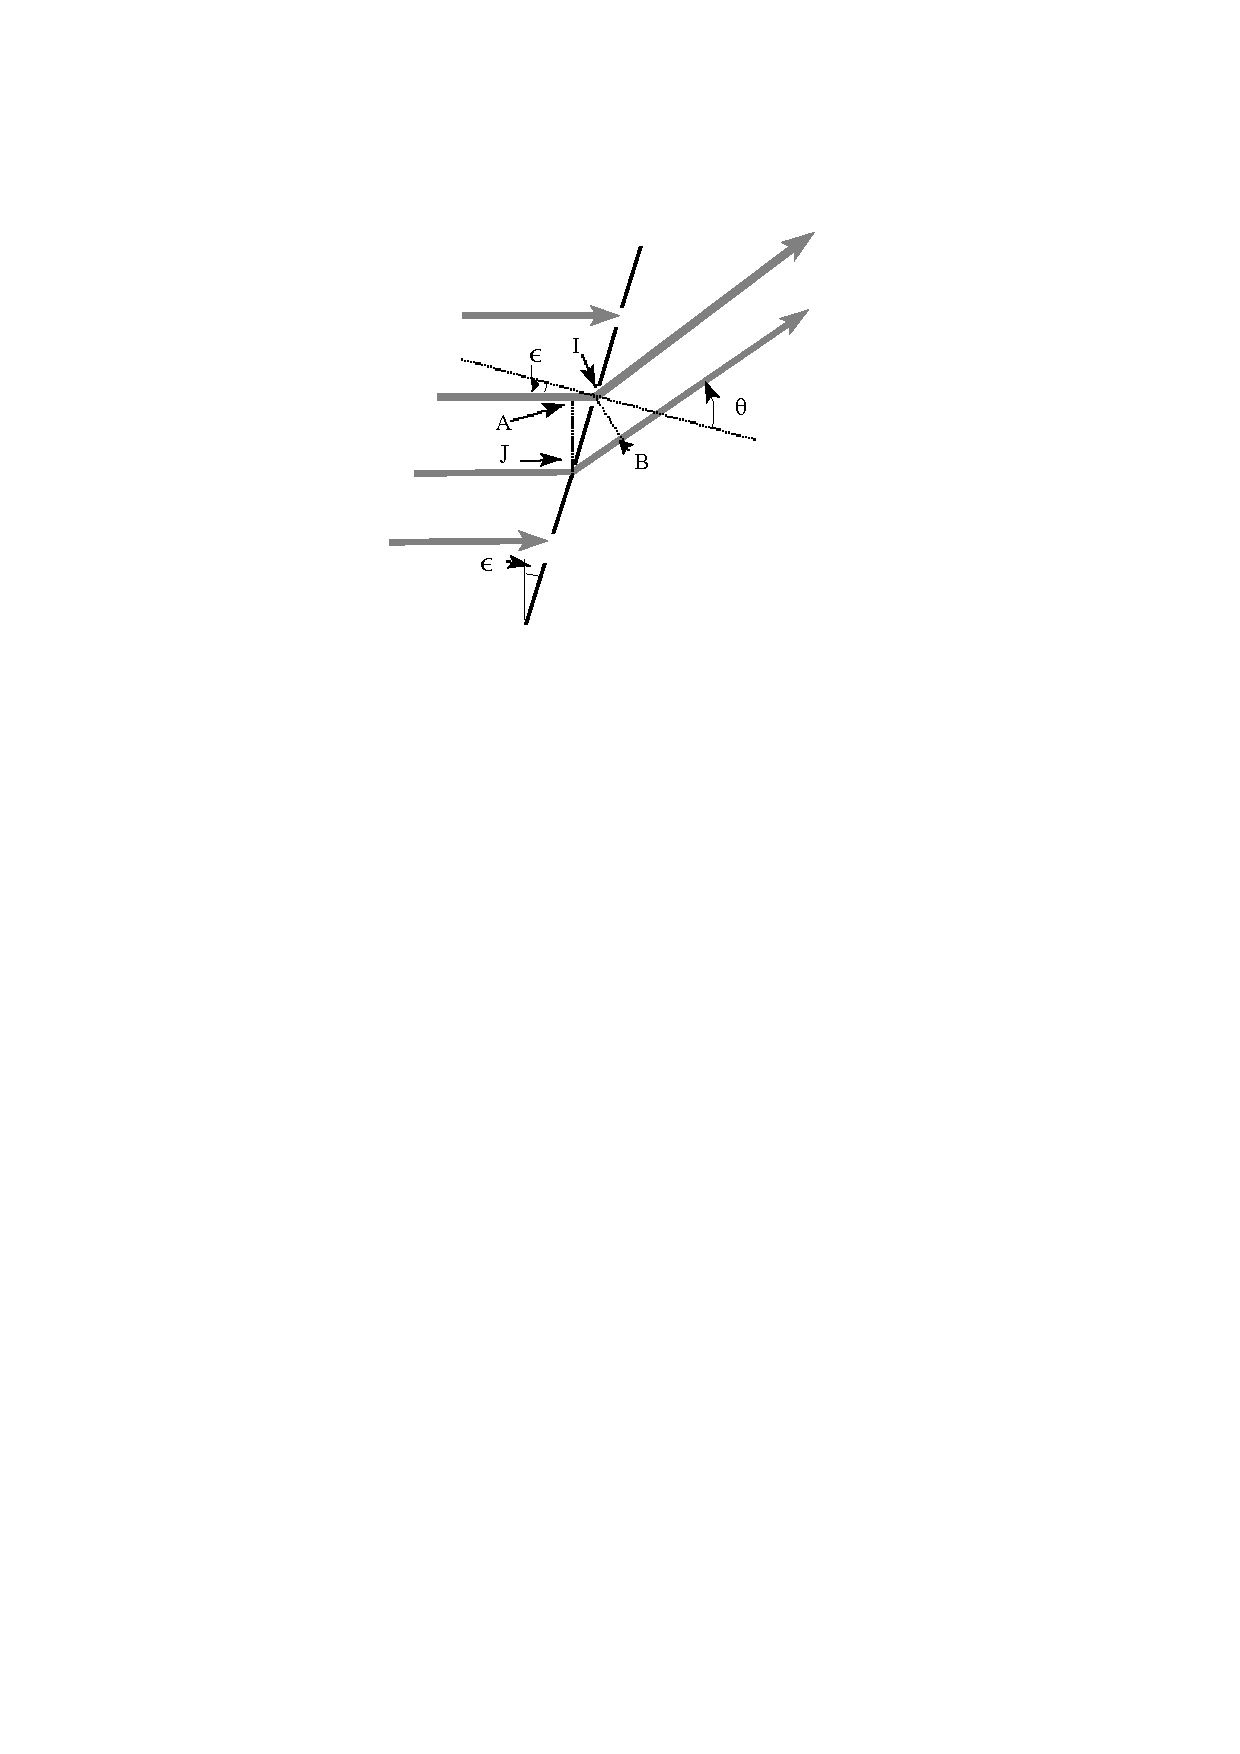
\includegraphics[scale = 0.7]{incidencia2.pdf}
		\caption{Incidencia no normal de la luz sobre la red}
		\label{fig:no normal}
	\end{minipage}
\end{figure}

Tal y como vemos en las \cref{eqn:interferencia,eqn:interferencia1}, la posición de los máximos depende de la longitud de onda. En particular, si la luz incidente no es monocromática veremos los patrones de interferencia para cada longitud de onda superimpuestos, \cref{fig:dispersion}. 

\begin{figure}
	\centering
	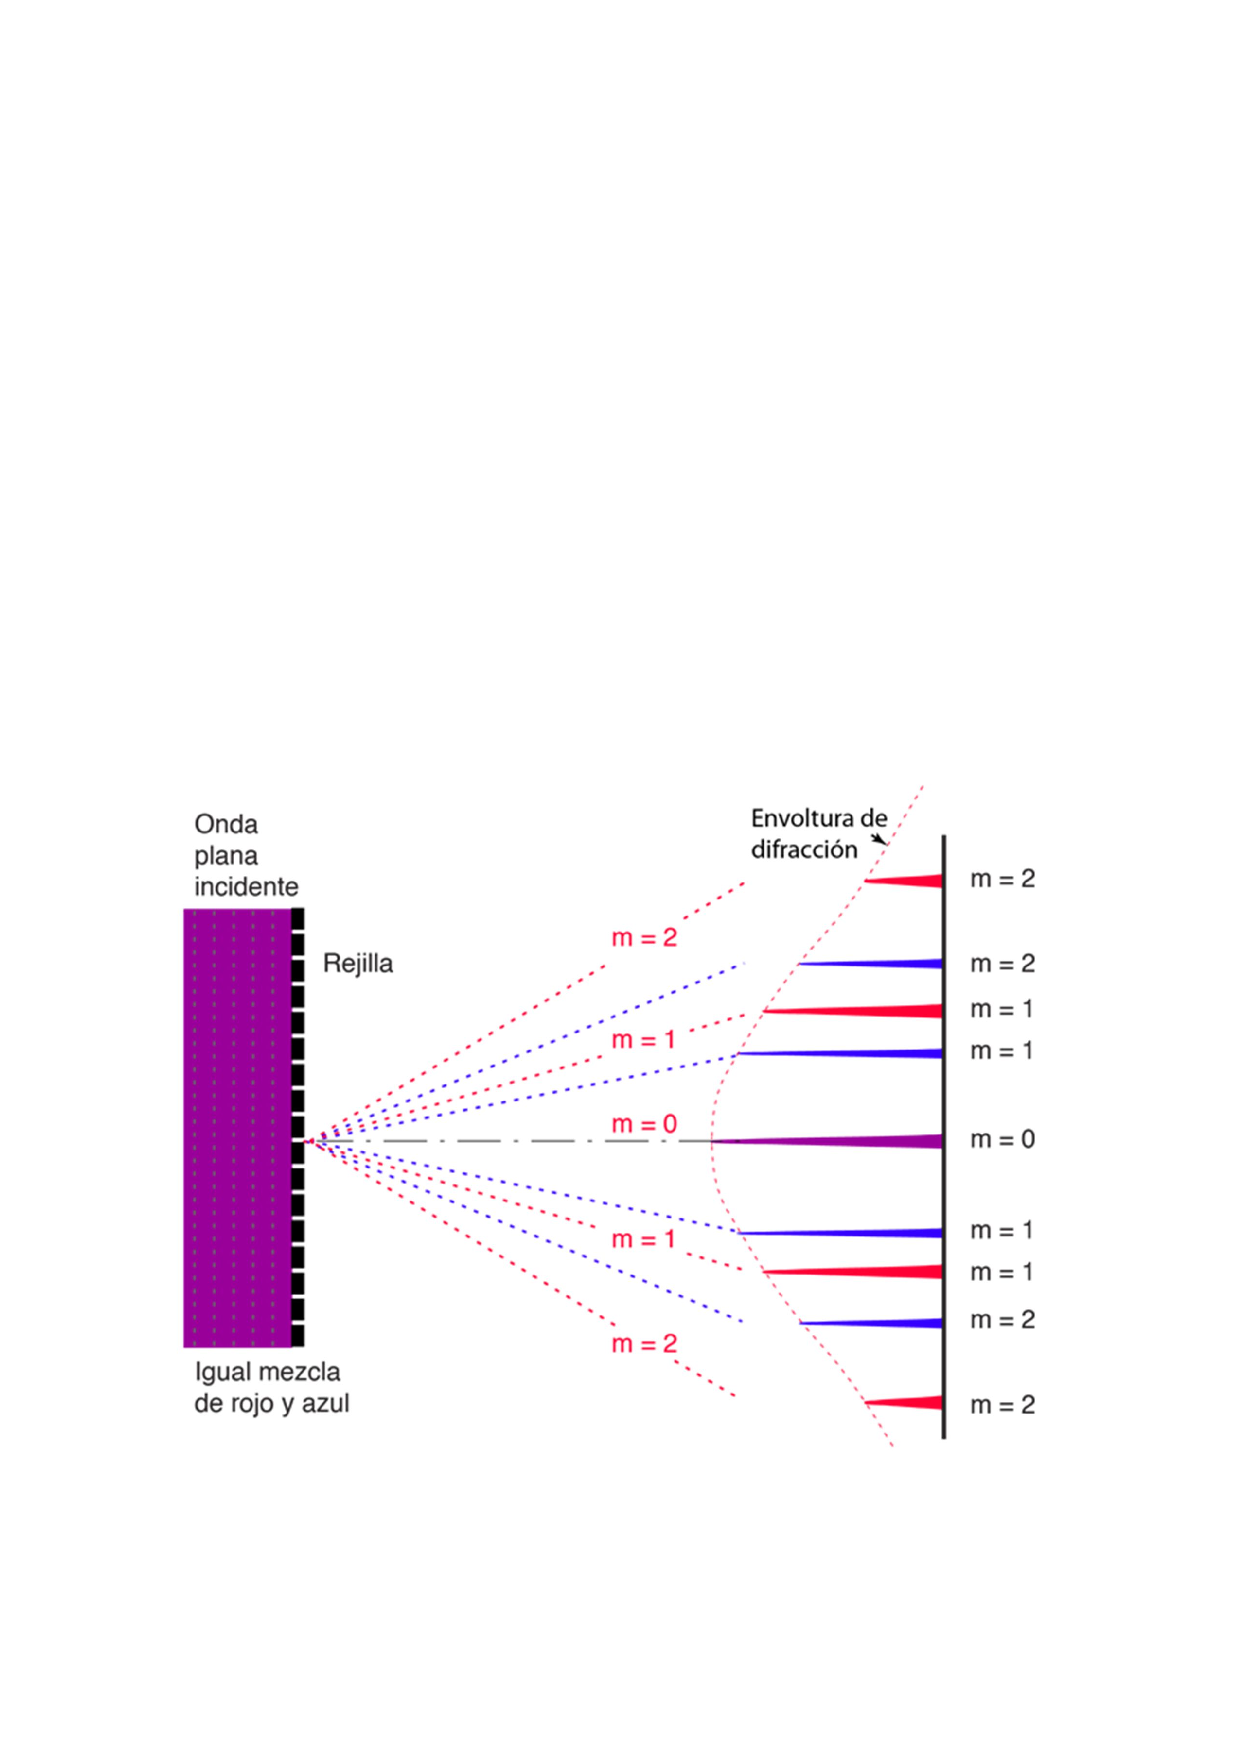
\includegraphics[scale = 0.5]{dispersion.pdf}
	\caption{Patrón de difracción con una fuente de luz no monocromática}
	\label{fig:dispersion}
\end{figure}

Si iluminamos la red de difracción con una funete de luz con un espectro determinado y medimos la posición de los picos de cada longitud de onda podemos, suponiendo conocido el parámetro \( a \), determinar las longitudes de onda del espectro. Esto es lo que haremos en la parte final con el espectro del hidrógeno, concretamente con la serie de Balmer. Estas son las líneas que corresponden a las transiciones atómicas de un estado cualquiera al primer estado excitado. En general, una transición del nivel \( n_i \) al nivel \( n_f \) implica una emisión o absorción de energia
\begin{equation*}
	\Delta E = E_1\left(\frac{1}{n_f^2} - \frac{1}{n_i^2}\right)
\end{equation*}
donde \( E_1 = \SI{-13.6}{eV} \) es la energia del nivel fundamental del hidrógeno. Esta energía se emite en forma de fotones con una lonigtud de onda que satisface \( \frac{hc}{\lambda} = -\Delta E \). Entonces, definiendo la constante de Rydberg como \( R_H = -\frac{E_1}{hc} \) llegamos a
\begin{equation*}
	\frac{1}{\lambda} = R_H\left(\frac{1}{n_f^2} - \frac{1}{n_i^2}\right)
\end{equation*}
por lo que
\begin{equation} \label{eqn:rydberg}
	R_H = \frac{n_i^2n_f^2}{(n_i^2 - n_f^2)\lambda}.
\end{equation}
Esta es la ecuación que usaremos para calcular la constante de RydbergEsta es la ecuación que usaremos para calcular la constante de Rydberg.

\section{Montaje experimental}
El montaje de esta práctica consiste de una fuente de luz (una lámpara de mercurio y otra dehidrógeno), una rendija y lente colimadora, una platina sobre la que se coloca la red de difracción, y un telescopio con un goniómetro para medir las desviaciones. Es necesario ajustar bien el telescopio, es decir, hacer coincidir las focales del ocular y el objetivo para que se pueda observar una imagen del infinito. Para ello se trata de enfocar un objeto lejano. Finalmente es importante que todos los elementos estén a la misma altura.

Igual como ocurre en la práctica 4, el orden en el que vemos las líneas cambia según si las observamos directamente o si las observamos a través del telescopio. Cuando las observamos con el telescopio vemos que las longitudes más cortas son las que menos se desvían, tal y como esperaríamos según la \cref{eqn:interferencia}, mientras que si lo observamos sin el telescopio vemos el patrón invertido: las longitudes más largas se desvían menos. Esto es porque cuando el ojo reconstruye el camino de los rayos los invierte, y cuando observamos por el telescopio la imagen se invierte otra vez por lo que vemos el patrón que esperaríamos.

Cuando giramos la red de difracción y por lo tanto alteramos el ángulo de incidencia, observamos que las líneas se acercan al máximo central hasta que llegan a un ángulo de desviación mínima y luego se vuelven a separar. El ángulo de desviación mínima además es diferente para varias longitudes de onda. Esto es llo que esperaríamos según la \cref{eqn:interferencia1}.

\section{Calibraje de la red}
Una vez hechas las observaciones cualitativas pertinentes pasamos al calibraje de la red. Esto consiste en determinar la separación entre rendijas \( a \). En primer lugar, pero, debemos garantizar que estamos en incidencia normal. Para ello ajustamos el colimador de manera que el haz que sale reflejado de la red vuelva a entrar por el diafragma. También es necesario ajustar la red de manera que sus surcos sean paralelos al haz colimado. Cuando sea así las líneas que vemos con el telescopio serán paralelas a la rendija. 

Una vez hecho esto anotamos la posición del máximo de orden zero, que servirá como ángulo de referencia. En nuestro caso, \( \theta_0 = \data{300.560}{0.008}{\degree} \). A continuación medimos la posición de otros máximos. Pudimos observar el máximo de orden 1 para todas las líneas del espectro del mercurio y el de orden \( 2 \) para las tres primeras. Los resultados se encuentran en el \cref{tab:datos Hg}.

Aunque hemos dispuesto la red intentando garantizar que la incidencia sea normal, podemos verificar que estamos en incidencia normal. En el laboratorio recogimos solamente datos para los máximos de uno de los dos lados, pero si dispusiésemos de los datos para ambos sabríamos que estamos en incidencia normal si las desviaciones fuesen simétricas respecto del ángulo de referencia. Es decir, si \( \theta_m \) es la desviación del máximo de orden \( m \) entonces, suponiendo incidencia normal, se verifica que 
\begin{equation*}
	a\sin{\theta_{-m}} =  -m\lambda = -a\sin{\theta_m} = a\sin{-\theta_m}
\end{equation*}
por lo que \( \theta_{-m} = -\theta_{m} \). Y si tenemos en cuenta el ángulo de referencia entonces debemos tener \( \theta_m - \theta_0 = -\theta_{-m} - \theta_0 \).

\begin{figure}[htb]
	\small \sffamily \centering
	%% Creator: Matplotlib, PGF backend
%%
%% To include the figure in your LaTeX document, write
%%   \input{<filename>.pgf}
%%
%% Make sure the required packages are loaded in your preamble
%%   \usepackage{pgf}
%%
%% Figures using additional raster images can only be included by \input if
%% they are in the same directory as the main LaTeX file. For loading figures
%% from other directories you can use the `import` package
%%   \usepackage{import}
%% and then include the figures with
%%   \import{<path to file>}{<filename>.pgf}
%%
%% Matplotlib used the following preamble
%%   \usepackage{siunitx}
%%   \usepackage[utf8]{inputenc}
%%   \usepackage{fontspec}
%%
\begingroup%
\makeatletter%
\begin{pgfpicture}%
\pgfpathrectangle{\pgfpointorigin}{\pgfqpoint{5.000000in}{3.500000in}}%
\pgfusepath{use as bounding box, clip}%
\begin{pgfscope}%
\pgfsetbuttcap%
\pgfsetmiterjoin%
\definecolor{currentfill}{rgb}{1.000000,1.000000,1.000000}%
\pgfsetfillcolor{currentfill}%
\pgfsetlinewidth{0.000000pt}%
\definecolor{currentstroke}{rgb}{1.000000,1.000000,1.000000}%
\pgfsetstrokecolor{currentstroke}%
\pgfsetdash{}{0pt}%
\pgfpathmoveto{\pgfqpoint{0.000000in}{0.000000in}}%
\pgfpathlineto{\pgfqpoint{5.000000in}{0.000000in}}%
\pgfpathlineto{\pgfqpoint{5.000000in}{3.500000in}}%
\pgfpathlineto{\pgfqpoint{0.000000in}{3.500000in}}%
\pgfpathclose%
\pgfusepath{fill}%
\end{pgfscope}%
\begin{pgfscope}%
\pgfsetbuttcap%
\pgfsetmiterjoin%
\definecolor{currentfill}{rgb}{1.000000,1.000000,1.000000}%
\pgfsetfillcolor{currentfill}%
\pgfsetlinewidth{0.000000pt}%
\definecolor{currentstroke}{rgb}{0.000000,0.000000,0.000000}%
\pgfsetstrokecolor{currentstroke}%
\pgfsetstrokeopacity{0.000000}%
\pgfsetdash{}{0pt}%
\pgfpathmoveto{\pgfqpoint{0.625000in}{0.437500in}}%
\pgfpathlineto{\pgfqpoint{4.500000in}{0.437500in}}%
\pgfpathlineto{\pgfqpoint{4.500000in}{3.080000in}}%
\pgfpathlineto{\pgfqpoint{0.625000in}{3.080000in}}%
\pgfpathclose%
\pgfusepath{fill}%
\end{pgfscope}%
\begin{pgfscope}%
\pgfpathrectangle{\pgfqpoint{0.625000in}{0.437500in}}{\pgfqpoint{3.875000in}{2.642500in}}%
\pgfusepath{clip}%
\pgfsetrectcap%
\pgfsetroundjoin%
\pgfsetlinewidth{0.803000pt}%
\definecolor{currentstroke}{rgb}{0.690196,0.690196,0.690196}%
\pgfsetstrokecolor{currentstroke}%
\pgfsetdash{}{0pt}%
\pgfpathmoveto{\pgfqpoint{0.801136in}{0.437500in}}%
\pgfpathlineto{\pgfqpoint{0.801136in}{3.080000in}}%
\pgfusepath{stroke}%
\end{pgfscope}%
\begin{pgfscope}%
\pgfsetbuttcap%
\pgfsetroundjoin%
\definecolor{currentfill}{rgb}{0.000000,0.000000,0.000000}%
\pgfsetfillcolor{currentfill}%
\pgfsetlinewidth{0.803000pt}%
\definecolor{currentstroke}{rgb}{0.000000,0.000000,0.000000}%
\pgfsetstrokecolor{currentstroke}%
\pgfsetdash{}{0pt}%
\pgfsys@defobject{currentmarker}{\pgfqpoint{0.000000in}{-0.048611in}}{\pgfqpoint{0.000000in}{0.000000in}}{%
\pgfpathmoveto{\pgfqpoint{0.000000in}{0.000000in}}%
\pgfpathlineto{\pgfqpoint{0.000000in}{-0.048611in}}%
\pgfusepath{stroke,fill}%
}%
\begin{pgfscope}%
\pgfsys@transformshift{0.801136in}{0.437500in}%
\pgfsys@useobject{currentmarker}{}%
\end{pgfscope}%
\end{pgfscope}%
\begin{pgfscope}%
\pgftext[x=0.801136in,y=0.340278in,,top]{\sffamily\fontsize{10.000000}{12.000000}\selectfont 0.0}%
\end{pgfscope}%
\begin{pgfscope}%
\pgfpathrectangle{\pgfqpoint{0.625000in}{0.437500in}}{\pgfqpoint{3.875000in}{2.642500in}}%
\pgfusepath{clip}%
\pgfsetrectcap%
\pgfsetroundjoin%
\pgfsetlinewidth{0.803000pt}%
\definecolor{currentstroke}{rgb}{0.690196,0.690196,0.690196}%
\pgfsetstrokecolor{currentstroke}%
\pgfsetdash{}{0pt}%
\pgfpathmoveto{\pgfqpoint{1.505896in}{0.437500in}}%
\pgfpathlineto{\pgfqpoint{1.505896in}{3.080000in}}%
\pgfusepath{stroke}%
\end{pgfscope}%
\begin{pgfscope}%
\pgfsetbuttcap%
\pgfsetroundjoin%
\definecolor{currentfill}{rgb}{0.000000,0.000000,0.000000}%
\pgfsetfillcolor{currentfill}%
\pgfsetlinewidth{0.803000pt}%
\definecolor{currentstroke}{rgb}{0.000000,0.000000,0.000000}%
\pgfsetstrokecolor{currentstroke}%
\pgfsetdash{}{0pt}%
\pgfsys@defobject{currentmarker}{\pgfqpoint{0.000000in}{-0.048611in}}{\pgfqpoint{0.000000in}{0.000000in}}{%
\pgfpathmoveto{\pgfqpoint{0.000000in}{0.000000in}}%
\pgfpathlineto{\pgfqpoint{0.000000in}{-0.048611in}}%
\pgfusepath{stroke,fill}%
}%
\begin{pgfscope}%
\pgfsys@transformshift{1.505896in}{0.437500in}%
\pgfsys@useobject{currentmarker}{}%
\end{pgfscope}%
\end{pgfscope}%
\begin{pgfscope}%
\pgftext[x=1.505896in,y=0.340278in,,top]{\sffamily\fontsize{10.000000}{12.000000}\selectfont 0.2}%
\end{pgfscope}%
\begin{pgfscope}%
\pgfpathrectangle{\pgfqpoint{0.625000in}{0.437500in}}{\pgfqpoint{3.875000in}{2.642500in}}%
\pgfusepath{clip}%
\pgfsetrectcap%
\pgfsetroundjoin%
\pgfsetlinewidth{0.803000pt}%
\definecolor{currentstroke}{rgb}{0.690196,0.690196,0.690196}%
\pgfsetstrokecolor{currentstroke}%
\pgfsetdash{}{0pt}%
\pgfpathmoveto{\pgfqpoint{2.210657in}{0.437500in}}%
\pgfpathlineto{\pgfqpoint{2.210657in}{3.080000in}}%
\pgfusepath{stroke}%
\end{pgfscope}%
\begin{pgfscope}%
\pgfsetbuttcap%
\pgfsetroundjoin%
\definecolor{currentfill}{rgb}{0.000000,0.000000,0.000000}%
\pgfsetfillcolor{currentfill}%
\pgfsetlinewidth{0.803000pt}%
\definecolor{currentstroke}{rgb}{0.000000,0.000000,0.000000}%
\pgfsetstrokecolor{currentstroke}%
\pgfsetdash{}{0pt}%
\pgfsys@defobject{currentmarker}{\pgfqpoint{0.000000in}{-0.048611in}}{\pgfqpoint{0.000000in}{0.000000in}}{%
\pgfpathmoveto{\pgfqpoint{0.000000in}{0.000000in}}%
\pgfpathlineto{\pgfqpoint{0.000000in}{-0.048611in}}%
\pgfusepath{stroke,fill}%
}%
\begin{pgfscope}%
\pgfsys@transformshift{2.210657in}{0.437500in}%
\pgfsys@useobject{currentmarker}{}%
\end{pgfscope}%
\end{pgfscope}%
\begin{pgfscope}%
\pgftext[x=2.210657in,y=0.340278in,,top]{\sffamily\fontsize{10.000000}{12.000000}\selectfont 0.4}%
\end{pgfscope}%
\begin{pgfscope}%
\pgfpathrectangle{\pgfqpoint{0.625000in}{0.437500in}}{\pgfqpoint{3.875000in}{2.642500in}}%
\pgfusepath{clip}%
\pgfsetrectcap%
\pgfsetroundjoin%
\pgfsetlinewidth{0.803000pt}%
\definecolor{currentstroke}{rgb}{0.690196,0.690196,0.690196}%
\pgfsetstrokecolor{currentstroke}%
\pgfsetdash{}{0pt}%
\pgfpathmoveto{\pgfqpoint{2.915417in}{0.437500in}}%
\pgfpathlineto{\pgfqpoint{2.915417in}{3.080000in}}%
\pgfusepath{stroke}%
\end{pgfscope}%
\begin{pgfscope}%
\pgfsetbuttcap%
\pgfsetroundjoin%
\definecolor{currentfill}{rgb}{0.000000,0.000000,0.000000}%
\pgfsetfillcolor{currentfill}%
\pgfsetlinewidth{0.803000pt}%
\definecolor{currentstroke}{rgb}{0.000000,0.000000,0.000000}%
\pgfsetstrokecolor{currentstroke}%
\pgfsetdash{}{0pt}%
\pgfsys@defobject{currentmarker}{\pgfqpoint{0.000000in}{-0.048611in}}{\pgfqpoint{0.000000in}{0.000000in}}{%
\pgfpathmoveto{\pgfqpoint{0.000000in}{0.000000in}}%
\pgfpathlineto{\pgfqpoint{0.000000in}{-0.048611in}}%
\pgfusepath{stroke,fill}%
}%
\begin{pgfscope}%
\pgfsys@transformshift{2.915417in}{0.437500in}%
\pgfsys@useobject{currentmarker}{}%
\end{pgfscope}%
\end{pgfscope}%
\begin{pgfscope}%
\pgftext[x=2.915417in,y=0.340278in,,top]{\sffamily\fontsize{10.000000}{12.000000}\selectfont 0.6}%
\end{pgfscope}%
\begin{pgfscope}%
\pgfpathrectangle{\pgfqpoint{0.625000in}{0.437500in}}{\pgfqpoint{3.875000in}{2.642500in}}%
\pgfusepath{clip}%
\pgfsetrectcap%
\pgfsetroundjoin%
\pgfsetlinewidth{0.803000pt}%
\definecolor{currentstroke}{rgb}{0.690196,0.690196,0.690196}%
\pgfsetstrokecolor{currentstroke}%
\pgfsetdash{}{0pt}%
\pgfpathmoveto{\pgfqpoint{3.620177in}{0.437500in}}%
\pgfpathlineto{\pgfqpoint{3.620177in}{3.080000in}}%
\pgfusepath{stroke}%
\end{pgfscope}%
\begin{pgfscope}%
\pgfsetbuttcap%
\pgfsetroundjoin%
\definecolor{currentfill}{rgb}{0.000000,0.000000,0.000000}%
\pgfsetfillcolor{currentfill}%
\pgfsetlinewidth{0.803000pt}%
\definecolor{currentstroke}{rgb}{0.000000,0.000000,0.000000}%
\pgfsetstrokecolor{currentstroke}%
\pgfsetdash{}{0pt}%
\pgfsys@defobject{currentmarker}{\pgfqpoint{0.000000in}{-0.048611in}}{\pgfqpoint{0.000000in}{0.000000in}}{%
\pgfpathmoveto{\pgfqpoint{0.000000in}{0.000000in}}%
\pgfpathlineto{\pgfqpoint{0.000000in}{-0.048611in}}%
\pgfusepath{stroke,fill}%
}%
\begin{pgfscope}%
\pgfsys@transformshift{3.620177in}{0.437500in}%
\pgfsys@useobject{currentmarker}{}%
\end{pgfscope}%
\end{pgfscope}%
\begin{pgfscope}%
\pgftext[x=3.620177in,y=0.340278in,,top]{\sffamily\fontsize{10.000000}{12.000000}\selectfont 0.8}%
\end{pgfscope}%
\begin{pgfscope}%
\pgfpathrectangle{\pgfqpoint{0.625000in}{0.437500in}}{\pgfqpoint{3.875000in}{2.642500in}}%
\pgfusepath{clip}%
\pgfsetrectcap%
\pgfsetroundjoin%
\pgfsetlinewidth{0.803000pt}%
\definecolor{currentstroke}{rgb}{0.690196,0.690196,0.690196}%
\pgfsetstrokecolor{currentstroke}%
\pgfsetdash{}{0pt}%
\pgfpathmoveto{\pgfqpoint{4.324937in}{0.437500in}}%
\pgfpathlineto{\pgfqpoint{4.324937in}{3.080000in}}%
\pgfusepath{stroke}%
\end{pgfscope}%
\begin{pgfscope}%
\pgfsetbuttcap%
\pgfsetroundjoin%
\definecolor{currentfill}{rgb}{0.000000,0.000000,0.000000}%
\pgfsetfillcolor{currentfill}%
\pgfsetlinewidth{0.803000pt}%
\definecolor{currentstroke}{rgb}{0.000000,0.000000,0.000000}%
\pgfsetstrokecolor{currentstroke}%
\pgfsetdash{}{0pt}%
\pgfsys@defobject{currentmarker}{\pgfqpoint{0.000000in}{-0.048611in}}{\pgfqpoint{0.000000in}{0.000000in}}{%
\pgfpathmoveto{\pgfqpoint{0.000000in}{0.000000in}}%
\pgfpathlineto{\pgfqpoint{0.000000in}{-0.048611in}}%
\pgfusepath{stroke,fill}%
}%
\begin{pgfscope}%
\pgfsys@transformshift{4.324937in}{0.437500in}%
\pgfsys@useobject{currentmarker}{}%
\end{pgfscope}%
\end{pgfscope}%
\begin{pgfscope}%
\pgftext[x=4.324937in,y=0.340278in,,top]{\sffamily\fontsize{10.000000}{12.000000}\selectfont 1.0}%
\end{pgfscope}%
\begin{pgfscope}%
\pgftext[x=2.562500in,y=0.161389in,,top]{\sffamily\fontsize{10.000000}{12.000000}\selectfont \( (\cos{\theta})^2 \)}%
\end{pgfscope}%
\begin{pgfscope}%
\pgfpathrectangle{\pgfqpoint{0.625000in}{0.437500in}}{\pgfqpoint{3.875000in}{2.642500in}}%
\pgfusepath{clip}%
\pgfsetrectcap%
\pgfsetroundjoin%
\pgfsetlinewidth{0.803000pt}%
\definecolor{currentstroke}{rgb}{0.690196,0.690196,0.690196}%
\pgfsetstrokecolor{currentstroke}%
\pgfsetdash{}{0pt}%
\pgfpathmoveto{\pgfqpoint{0.625000in}{0.557614in}}%
\pgfpathlineto{\pgfqpoint{4.500000in}{0.557614in}}%
\pgfusepath{stroke}%
\end{pgfscope}%
\begin{pgfscope}%
\pgfsetbuttcap%
\pgfsetroundjoin%
\definecolor{currentfill}{rgb}{0.000000,0.000000,0.000000}%
\pgfsetfillcolor{currentfill}%
\pgfsetlinewidth{0.803000pt}%
\definecolor{currentstroke}{rgb}{0.000000,0.000000,0.000000}%
\pgfsetstrokecolor{currentstroke}%
\pgfsetdash{}{0pt}%
\pgfsys@defobject{currentmarker}{\pgfqpoint{-0.048611in}{0.000000in}}{\pgfqpoint{0.000000in}{0.000000in}}{%
\pgfpathmoveto{\pgfqpoint{0.000000in}{0.000000in}}%
\pgfpathlineto{\pgfqpoint{-0.048611in}{0.000000in}}%
\pgfusepath{stroke,fill}%
}%
\begin{pgfscope}%
\pgfsys@transformshift{0.625000in}{0.557614in}%
\pgfsys@useobject{currentmarker}{}%
\end{pgfscope}%
\end{pgfscope}%
\begin{pgfscope}%
\pgftext[x=0.350278in,y=0.509419in,left,base]{\sffamily\fontsize{10.000000}{12.000000}\selectfont 0.0}%
\end{pgfscope}%
\begin{pgfscope}%
\pgfpathrectangle{\pgfqpoint{0.625000in}{0.437500in}}{\pgfqpoint{3.875000in}{2.642500in}}%
\pgfusepath{clip}%
\pgfsetrectcap%
\pgfsetroundjoin%
\pgfsetlinewidth{0.803000pt}%
\definecolor{currentstroke}{rgb}{0.690196,0.690196,0.690196}%
\pgfsetstrokecolor{currentstroke}%
\pgfsetdash{}{0pt}%
\pgfpathmoveto{\pgfqpoint{0.625000in}{1.033311in}}%
\pgfpathlineto{\pgfqpoint{4.500000in}{1.033311in}}%
\pgfusepath{stroke}%
\end{pgfscope}%
\begin{pgfscope}%
\pgfsetbuttcap%
\pgfsetroundjoin%
\definecolor{currentfill}{rgb}{0.000000,0.000000,0.000000}%
\pgfsetfillcolor{currentfill}%
\pgfsetlinewidth{0.803000pt}%
\definecolor{currentstroke}{rgb}{0.000000,0.000000,0.000000}%
\pgfsetstrokecolor{currentstroke}%
\pgfsetdash{}{0pt}%
\pgfsys@defobject{currentmarker}{\pgfqpoint{-0.048611in}{0.000000in}}{\pgfqpoint{0.000000in}{0.000000in}}{%
\pgfpathmoveto{\pgfqpoint{0.000000in}{0.000000in}}%
\pgfpathlineto{\pgfqpoint{-0.048611in}{0.000000in}}%
\pgfusepath{stroke,fill}%
}%
\begin{pgfscope}%
\pgfsys@transformshift{0.625000in}{1.033311in}%
\pgfsys@useobject{currentmarker}{}%
\end{pgfscope}%
\end{pgfscope}%
\begin{pgfscope}%
\pgftext[x=0.350278in,y=0.985117in,left,base]{\sffamily\fontsize{10.000000}{12.000000}\selectfont 0.2}%
\end{pgfscope}%
\begin{pgfscope}%
\pgfpathrectangle{\pgfqpoint{0.625000in}{0.437500in}}{\pgfqpoint{3.875000in}{2.642500in}}%
\pgfusepath{clip}%
\pgfsetrectcap%
\pgfsetroundjoin%
\pgfsetlinewidth{0.803000pt}%
\definecolor{currentstroke}{rgb}{0.690196,0.690196,0.690196}%
\pgfsetstrokecolor{currentstroke}%
\pgfsetdash{}{0pt}%
\pgfpathmoveto{\pgfqpoint{0.625000in}{1.509009in}}%
\pgfpathlineto{\pgfqpoint{4.500000in}{1.509009in}}%
\pgfusepath{stroke}%
\end{pgfscope}%
\begin{pgfscope}%
\pgfsetbuttcap%
\pgfsetroundjoin%
\definecolor{currentfill}{rgb}{0.000000,0.000000,0.000000}%
\pgfsetfillcolor{currentfill}%
\pgfsetlinewidth{0.803000pt}%
\definecolor{currentstroke}{rgb}{0.000000,0.000000,0.000000}%
\pgfsetstrokecolor{currentstroke}%
\pgfsetdash{}{0pt}%
\pgfsys@defobject{currentmarker}{\pgfqpoint{-0.048611in}{0.000000in}}{\pgfqpoint{0.000000in}{0.000000in}}{%
\pgfpathmoveto{\pgfqpoint{0.000000in}{0.000000in}}%
\pgfpathlineto{\pgfqpoint{-0.048611in}{0.000000in}}%
\pgfusepath{stroke,fill}%
}%
\begin{pgfscope}%
\pgfsys@transformshift{0.625000in}{1.509009in}%
\pgfsys@useobject{currentmarker}{}%
\end{pgfscope}%
\end{pgfscope}%
\begin{pgfscope}%
\pgftext[x=0.350278in,y=1.460814in,left,base]{\sffamily\fontsize{10.000000}{12.000000}\selectfont 0.4}%
\end{pgfscope}%
\begin{pgfscope}%
\pgfpathrectangle{\pgfqpoint{0.625000in}{0.437500in}}{\pgfqpoint{3.875000in}{2.642500in}}%
\pgfusepath{clip}%
\pgfsetrectcap%
\pgfsetroundjoin%
\pgfsetlinewidth{0.803000pt}%
\definecolor{currentstroke}{rgb}{0.690196,0.690196,0.690196}%
\pgfsetstrokecolor{currentstroke}%
\pgfsetdash{}{0pt}%
\pgfpathmoveto{\pgfqpoint{0.625000in}{1.984706in}}%
\pgfpathlineto{\pgfqpoint{4.500000in}{1.984706in}}%
\pgfusepath{stroke}%
\end{pgfscope}%
\begin{pgfscope}%
\pgfsetbuttcap%
\pgfsetroundjoin%
\definecolor{currentfill}{rgb}{0.000000,0.000000,0.000000}%
\pgfsetfillcolor{currentfill}%
\pgfsetlinewidth{0.803000pt}%
\definecolor{currentstroke}{rgb}{0.000000,0.000000,0.000000}%
\pgfsetstrokecolor{currentstroke}%
\pgfsetdash{}{0pt}%
\pgfsys@defobject{currentmarker}{\pgfqpoint{-0.048611in}{0.000000in}}{\pgfqpoint{0.000000in}{0.000000in}}{%
\pgfpathmoveto{\pgfqpoint{0.000000in}{0.000000in}}%
\pgfpathlineto{\pgfqpoint{-0.048611in}{0.000000in}}%
\pgfusepath{stroke,fill}%
}%
\begin{pgfscope}%
\pgfsys@transformshift{0.625000in}{1.984706in}%
\pgfsys@useobject{currentmarker}{}%
\end{pgfscope}%
\end{pgfscope}%
\begin{pgfscope}%
\pgftext[x=0.350278in,y=1.936512in,left,base]{\sffamily\fontsize{10.000000}{12.000000}\selectfont 0.6}%
\end{pgfscope}%
\begin{pgfscope}%
\pgfpathrectangle{\pgfqpoint{0.625000in}{0.437500in}}{\pgfqpoint{3.875000in}{2.642500in}}%
\pgfusepath{clip}%
\pgfsetrectcap%
\pgfsetroundjoin%
\pgfsetlinewidth{0.803000pt}%
\definecolor{currentstroke}{rgb}{0.690196,0.690196,0.690196}%
\pgfsetstrokecolor{currentstroke}%
\pgfsetdash{}{0pt}%
\pgfpathmoveto{\pgfqpoint{0.625000in}{2.460404in}}%
\pgfpathlineto{\pgfqpoint{4.500000in}{2.460404in}}%
\pgfusepath{stroke}%
\end{pgfscope}%
\begin{pgfscope}%
\pgfsetbuttcap%
\pgfsetroundjoin%
\definecolor{currentfill}{rgb}{0.000000,0.000000,0.000000}%
\pgfsetfillcolor{currentfill}%
\pgfsetlinewidth{0.803000pt}%
\definecolor{currentstroke}{rgb}{0.000000,0.000000,0.000000}%
\pgfsetstrokecolor{currentstroke}%
\pgfsetdash{}{0pt}%
\pgfsys@defobject{currentmarker}{\pgfqpoint{-0.048611in}{0.000000in}}{\pgfqpoint{0.000000in}{0.000000in}}{%
\pgfpathmoveto{\pgfqpoint{0.000000in}{0.000000in}}%
\pgfpathlineto{\pgfqpoint{-0.048611in}{0.000000in}}%
\pgfusepath{stroke,fill}%
}%
\begin{pgfscope}%
\pgfsys@transformshift{0.625000in}{2.460404in}%
\pgfsys@useobject{currentmarker}{}%
\end{pgfscope}%
\end{pgfscope}%
\begin{pgfscope}%
\pgftext[x=0.350278in,y=2.412209in,left,base]{\sffamily\fontsize{10.000000}{12.000000}\selectfont 0.8}%
\end{pgfscope}%
\begin{pgfscope}%
\pgfpathrectangle{\pgfqpoint{0.625000in}{0.437500in}}{\pgfqpoint{3.875000in}{2.642500in}}%
\pgfusepath{clip}%
\pgfsetrectcap%
\pgfsetroundjoin%
\pgfsetlinewidth{0.803000pt}%
\definecolor{currentstroke}{rgb}{0.690196,0.690196,0.690196}%
\pgfsetstrokecolor{currentstroke}%
\pgfsetdash{}{0pt}%
\pgfpathmoveto{\pgfqpoint{0.625000in}{2.936101in}}%
\pgfpathlineto{\pgfqpoint{4.500000in}{2.936101in}}%
\pgfusepath{stroke}%
\end{pgfscope}%
\begin{pgfscope}%
\pgfsetbuttcap%
\pgfsetroundjoin%
\definecolor{currentfill}{rgb}{0.000000,0.000000,0.000000}%
\pgfsetfillcolor{currentfill}%
\pgfsetlinewidth{0.803000pt}%
\definecolor{currentstroke}{rgb}{0.000000,0.000000,0.000000}%
\pgfsetstrokecolor{currentstroke}%
\pgfsetdash{}{0pt}%
\pgfsys@defobject{currentmarker}{\pgfqpoint{-0.048611in}{0.000000in}}{\pgfqpoint{0.000000in}{0.000000in}}{%
\pgfpathmoveto{\pgfqpoint{0.000000in}{0.000000in}}%
\pgfpathlineto{\pgfqpoint{-0.048611in}{0.000000in}}%
\pgfusepath{stroke,fill}%
}%
\begin{pgfscope}%
\pgfsys@transformshift{0.625000in}{2.936101in}%
\pgfsys@useobject{currentmarker}{}%
\end{pgfscope}%
\end{pgfscope}%
\begin{pgfscope}%
\pgftext[x=0.350278in,y=2.887907in,left,base]{\sffamily\fontsize{10.000000}{12.000000}\selectfont 1.0}%
\end{pgfscope}%
\begin{pgfscope}%
\pgftext[x=0.294722in,y=1.758750in,,bottom,rotate=90.000000]{\sffamily\fontsize{10.000000}{12.000000}\selectfont \( I \, (\si{\mW}) \)}%
\end{pgfscope}%
\begin{pgfscope}%
\pgfpathrectangle{\pgfqpoint{0.625000in}{0.437500in}}{\pgfqpoint{3.875000in}{2.642500in}}%
\pgfusepath{clip}%
\pgfsetbuttcap%
\pgfsetroundjoin%
\definecolor{currentfill}{rgb}{0.678431,0.847059,0.901961}%
\pgfsetfillcolor{currentfill}%
\pgfsetlinewidth{1.003750pt}%
\definecolor{currentstroke}{rgb}{0.121569,0.466667,0.705882}%
\pgfsetstrokecolor{currentstroke}%
\pgfsetdash{}{0pt}%
\pgfsys@defobject{currentmarker}{\pgfqpoint{-0.048611in}{-0.048611in}}{\pgfqpoint{0.048611in}{0.048611in}}{%
\pgfpathmoveto{\pgfqpoint{-0.048611in}{0.000000in}}%
\pgfpathlineto{\pgfqpoint{0.048611in}{0.000000in}}%
\pgfpathmoveto{\pgfqpoint{0.000000in}{-0.048611in}}%
\pgfpathlineto{\pgfqpoint{0.000000in}{0.048611in}}%
\pgfusepath{stroke,fill}%
}%
\begin{pgfscope}%
\pgfsys@transformshift{0.810788in}{0.557614in}%
\pgfsys@useobject{currentmarker}{}%
\end{pgfscope}%
\begin{pgfscope}%
\pgfsys@transformshift{0.979451in}{0.700323in}%
\pgfsys@useobject{currentmarker}{}%
\end{pgfscope}%
\begin{pgfscope}%
\pgfsys@transformshift{1.339118in}{0.914387in}%
\pgfsys@useobject{currentmarker}{}%
\end{pgfscope}%
\begin{pgfscope}%
\pgfsys@transformshift{1.846407in}{1.271160in}%
\pgfsys@useobject{currentmarker}{}%
\end{pgfscope}%
\begin{pgfscope}%
\pgfsys@transformshift{2.440133in}{1.651718in}%
\pgfsys@useobject{currentmarker}{}%
\end{pgfscope}%
\begin{pgfscope}%
\pgfsys@transformshift{3.048682in}{2.103631in}%
\pgfsys@useobject{currentmarker}{}%
\end{pgfscope}%
\begin{pgfscope}%
\pgfsys@transformshift{3.598656in}{2.436619in}%
\pgfsys@useobject{currentmarker}{}%
\end{pgfscope}%
\begin{pgfscope}%
\pgfsys@transformshift{4.023718in}{2.722038in}%
\pgfsys@useobject{currentmarker}{}%
\end{pgfscope}%
\begin{pgfscope}%
\pgfsys@transformshift{4.272601in}{2.912317in}%
\pgfsys@useobject{currentmarker}{}%
\end{pgfscope}%
\begin{pgfscope}%
\pgfsys@transformshift{4.146622in}{2.817177in}%
\pgfsys@useobject{currentmarker}{}%
\end{pgfscope}%
\begin{pgfscope}%
\pgfsys@transformshift{4.088887in}{2.769607in}%
\pgfsys@useobject{currentmarker}{}%
\end{pgfscope}%
\begin{pgfscope}%
\pgfsys@transformshift{4.196642in}{2.864747in}%
\pgfsys@useobject{currentmarker}{}%
\end{pgfscope}%
\begin{pgfscope}%
\pgfsys@transformshift{4.238703in}{2.888532in}%
\pgfsys@useobject{currentmarker}{}%
\end{pgfscope}%
\begin{pgfscope}%
\pgfsys@transformshift{4.298170in}{2.936101in}%
\pgfsys@useobject{currentmarker}{}%
\end{pgfscope}%
\begin{pgfscope}%
\pgfsys@transformshift{4.315285in}{2.936101in}%
\pgfsys@useobject{currentmarker}{}%
\end{pgfscope}%
\begin{pgfscope}%
\pgfsys@transformshift{4.323864in}{2.959886in}%
\pgfsys@useobject{currentmarker}{}%
\end{pgfscope}%
\begin{pgfscope}%
\pgfsys@transformshift{4.323864in}{2.959886in}%
\pgfsys@useobject{currentmarker}{}%
\end{pgfscope}%
\begin{pgfscope}%
\pgfsys@transformshift{4.315285in}{2.936101in}%
\pgfsys@useobject{currentmarker}{}%
\end{pgfscope}%
\begin{pgfscope}%
\pgfsys@transformshift{4.298170in}{2.936101in}%
\pgfsys@useobject{currentmarker}{}%
\end{pgfscope}%
\begin{pgfscope}%
\pgfsys@transformshift{4.272601in}{2.912317in}%
\pgfsys@useobject{currentmarker}{}%
\end{pgfscope}%
\begin{pgfscope}%
\pgfsys@transformshift{4.238703in}{2.888532in}%
\pgfsys@useobject{currentmarker}{}%
\end{pgfscope}%
\begin{pgfscope}%
\pgfsys@transformshift{4.196642in}{2.864747in}%
\pgfsys@useobject{currentmarker}{}%
\end{pgfscope}%
\begin{pgfscope}%
\pgfsys@transformshift{4.146622in}{2.840962in}%
\pgfsys@useobject{currentmarker}{}%
\end{pgfscope}%
\begin{pgfscope}%
\pgfsys@transformshift{4.088887in}{2.793392in}%
\pgfsys@useobject{currentmarker}{}%
\end{pgfscope}%
\begin{pgfscope}%
\pgfsys@transformshift{4.023718in}{2.745822in}%
\pgfsys@useobject{currentmarker}{}%
\end{pgfscope}%
\begin{pgfscope}%
\pgfsys@transformshift{3.951433in}{2.698253in}%
\pgfsys@useobject{currentmarker}{}%
\end{pgfscope}%
\begin{pgfscope}%
\pgfsys@transformshift{3.872384in}{2.650683in}%
\pgfsys@useobject{currentmarker}{}%
\end{pgfscope}%
\begin{pgfscope}%
\pgfsys@transformshift{3.786955in}{2.603113in}%
\pgfsys@useobject{currentmarker}{}%
\end{pgfscope}%
\begin{pgfscope}%
\pgfsys@transformshift{3.279666in}{2.270125in}%
\pgfsys@useobject{currentmarker}{}%
\end{pgfscope}%
\begin{pgfscope}%
\pgfsys@transformshift{2.685941in}{1.889567in}%
\pgfsys@useobject{currentmarker}{}%
\end{pgfscope}%
\begin{pgfscope}%
\pgfsys@transformshift{2.077391in}{1.461439in}%
\pgfsys@useobject{currentmarker}{}%
\end{pgfscope}%
\begin{pgfscope}%
\pgfsys@transformshift{1.527418in}{1.057096in}%
\pgfsys@useobject{currentmarker}{}%
\end{pgfscope}%
\begin{pgfscope}%
\pgfsys@transformshift{1.102355in}{0.771678in}%
\pgfsys@useobject{currentmarker}{}%
\end{pgfscope}%
\begin{pgfscope}%
\pgfsys@transformshift{0.853472in}{0.605183in}%
\pgfsys@useobject{currentmarker}{}%
\end{pgfscope}%
\begin{pgfscope}%
\pgfsys@transformshift{0.810788in}{0.557614in}%
\pgfsys@useobject{currentmarker}{}%
\end{pgfscope}%
\end{pgfscope}%
\begin{pgfscope}%
\pgfpathrectangle{\pgfqpoint{0.625000in}{0.437500in}}{\pgfqpoint{3.875000in}{2.642500in}}%
\pgfusepath{clip}%
\pgfsetbuttcap%
\pgfsetroundjoin%
\pgfsetlinewidth{1.003750pt}%
\definecolor{currentstroke}{rgb}{0.854902,0.439216,0.839216}%
\pgfsetstrokecolor{currentstroke}%
\pgfsetdash{{3.700000pt}{1.600000pt}}{0.000000pt}%
\pgfpathmoveto{\pgfqpoint{0.801136in}{0.567466in}}%
\pgfpathlineto{\pgfqpoint{0.836374in}{0.591301in}}%
\pgfpathlineto{\pgfqpoint{0.871612in}{0.615137in}}%
\pgfpathlineto{\pgfqpoint{0.906850in}{0.638973in}}%
\pgfpathlineto{\pgfqpoint{0.942088in}{0.662808in}}%
\pgfpathlineto{\pgfqpoint{0.977326in}{0.686644in}}%
\pgfpathlineto{\pgfqpoint{1.012564in}{0.710479in}}%
\pgfpathlineto{\pgfqpoint{1.047802in}{0.734315in}}%
\pgfpathlineto{\pgfqpoint{1.083040in}{0.758151in}}%
\pgfpathlineto{\pgfqpoint{1.118278in}{0.781986in}}%
\pgfpathlineto{\pgfqpoint{1.153516in}{0.805822in}}%
\pgfpathlineto{\pgfqpoint{1.188754in}{0.829657in}}%
\pgfpathlineto{\pgfqpoint{1.223992in}{0.853493in}}%
\pgfpathlineto{\pgfqpoint{1.259230in}{0.877329in}}%
\pgfpathlineto{\pgfqpoint{1.294468in}{0.901164in}}%
\pgfpathlineto{\pgfqpoint{1.329706in}{0.925000in}}%
\pgfpathlineto{\pgfqpoint{1.364944in}{0.948836in}}%
\pgfpathlineto{\pgfqpoint{1.400182in}{0.972671in}}%
\pgfpathlineto{\pgfqpoint{1.435420in}{0.996507in}}%
\pgfpathlineto{\pgfqpoint{1.470658in}{1.020342in}}%
\pgfpathlineto{\pgfqpoint{1.505896in}{1.044178in}}%
\pgfpathlineto{\pgfqpoint{1.541134in}{1.068014in}}%
\pgfpathlineto{\pgfqpoint{1.576372in}{1.091849in}}%
\pgfpathlineto{\pgfqpoint{1.611610in}{1.115685in}}%
\pgfpathlineto{\pgfqpoint{1.646849in}{1.139520in}}%
\pgfpathlineto{\pgfqpoint{1.682087in}{1.163356in}}%
\pgfpathlineto{\pgfqpoint{1.717325in}{1.187192in}}%
\pgfpathlineto{\pgfqpoint{1.752563in}{1.211027in}}%
\pgfpathlineto{\pgfqpoint{1.787801in}{1.234863in}}%
\pgfpathlineto{\pgfqpoint{1.823039in}{1.258698in}}%
\pgfpathlineto{\pgfqpoint{1.858277in}{1.282534in}}%
\pgfpathlineto{\pgfqpoint{1.893515in}{1.306370in}}%
\pgfpathlineto{\pgfqpoint{1.928753in}{1.330205in}}%
\pgfpathlineto{\pgfqpoint{1.963991in}{1.354041in}}%
\pgfpathlineto{\pgfqpoint{1.999229in}{1.377876in}}%
\pgfpathlineto{\pgfqpoint{2.034467in}{1.401712in}}%
\pgfpathlineto{\pgfqpoint{2.069705in}{1.425548in}}%
\pgfpathlineto{\pgfqpoint{2.104943in}{1.449383in}}%
\pgfpathlineto{\pgfqpoint{2.140181in}{1.473219in}}%
\pgfpathlineto{\pgfqpoint{2.175419in}{1.497054in}}%
\pgfpathlineto{\pgfqpoint{2.210657in}{1.520890in}}%
\pgfpathlineto{\pgfqpoint{2.245895in}{1.544726in}}%
\pgfpathlineto{\pgfqpoint{2.281133in}{1.568561in}}%
\pgfpathlineto{\pgfqpoint{2.316371in}{1.592397in}}%
\pgfpathlineto{\pgfqpoint{2.351609in}{1.616232in}}%
\pgfpathlineto{\pgfqpoint{2.386847in}{1.640068in}}%
\pgfpathlineto{\pgfqpoint{2.422085in}{1.663904in}}%
\pgfpathlineto{\pgfqpoint{2.457323in}{1.687739in}}%
\pgfpathlineto{\pgfqpoint{2.492561in}{1.711575in}}%
\pgfpathlineto{\pgfqpoint{2.527799in}{1.735410in}}%
\pgfpathlineto{\pgfqpoint{2.563037in}{1.759246in}}%
\pgfpathlineto{\pgfqpoint{2.598275in}{1.783082in}}%
\pgfpathlineto{\pgfqpoint{2.633513in}{1.806917in}}%
\pgfpathlineto{\pgfqpoint{2.668751in}{1.830753in}}%
\pgfpathlineto{\pgfqpoint{2.703989in}{1.854588in}}%
\pgfpathlineto{\pgfqpoint{2.739227in}{1.878424in}}%
\pgfpathlineto{\pgfqpoint{2.774465in}{1.902260in}}%
\pgfpathlineto{\pgfqpoint{2.809703in}{1.926095in}}%
\pgfpathlineto{\pgfqpoint{2.844941in}{1.949931in}}%
\pgfpathlineto{\pgfqpoint{2.880179in}{1.973767in}}%
\pgfpathlineto{\pgfqpoint{2.915417in}{1.997602in}}%
\pgfpathlineto{\pgfqpoint{2.950655in}{2.021438in}}%
\pgfpathlineto{\pgfqpoint{2.985893in}{2.045273in}}%
\pgfpathlineto{\pgfqpoint{3.021131in}{2.069109in}}%
\pgfpathlineto{\pgfqpoint{3.056369in}{2.092945in}}%
\pgfpathlineto{\pgfqpoint{3.091607in}{2.116780in}}%
\pgfpathlineto{\pgfqpoint{3.126845in}{2.140616in}}%
\pgfpathlineto{\pgfqpoint{3.162083in}{2.164451in}}%
\pgfpathlineto{\pgfqpoint{3.197321in}{2.188287in}}%
\pgfpathlineto{\pgfqpoint{3.232559in}{2.212123in}}%
\pgfpathlineto{\pgfqpoint{3.267797in}{2.235958in}}%
\pgfpathlineto{\pgfqpoint{3.303035in}{2.259794in}}%
\pgfpathlineto{\pgfqpoint{3.338273in}{2.283629in}}%
\pgfpathlineto{\pgfqpoint{3.373511in}{2.307465in}}%
\pgfpathlineto{\pgfqpoint{3.408749in}{2.331301in}}%
\pgfpathlineto{\pgfqpoint{3.443987in}{2.355136in}}%
\pgfpathlineto{\pgfqpoint{3.479225in}{2.378972in}}%
\pgfpathlineto{\pgfqpoint{3.514463in}{2.402807in}}%
\pgfpathlineto{\pgfqpoint{3.549701in}{2.426643in}}%
\pgfpathlineto{\pgfqpoint{3.584939in}{2.450479in}}%
\pgfpathlineto{\pgfqpoint{3.620177in}{2.474314in}}%
\pgfpathlineto{\pgfqpoint{3.655415in}{2.498150in}}%
\pgfpathlineto{\pgfqpoint{3.690653in}{2.521985in}}%
\pgfpathlineto{\pgfqpoint{3.725891in}{2.545821in}}%
\pgfpathlineto{\pgfqpoint{3.761129in}{2.569657in}}%
\pgfpathlineto{\pgfqpoint{3.796367in}{2.593492in}}%
\pgfpathlineto{\pgfqpoint{3.831605in}{2.617328in}}%
\pgfpathlineto{\pgfqpoint{3.866843in}{2.641163in}}%
\pgfpathlineto{\pgfqpoint{3.902081in}{2.664999in}}%
\pgfpathlineto{\pgfqpoint{3.937319in}{2.688835in}}%
\pgfpathlineto{\pgfqpoint{3.972557in}{2.712670in}}%
\pgfpathlineto{\pgfqpoint{4.007795in}{2.736506in}}%
\pgfpathlineto{\pgfqpoint{4.043033in}{2.760341in}}%
\pgfpathlineto{\pgfqpoint{4.078271in}{2.784177in}}%
\pgfpathlineto{\pgfqpoint{4.113509in}{2.808013in}}%
\pgfpathlineto{\pgfqpoint{4.148747in}{2.831848in}}%
\pgfpathlineto{\pgfqpoint{4.183985in}{2.855684in}}%
\pgfpathlineto{\pgfqpoint{4.219223in}{2.879519in}}%
\pgfpathlineto{\pgfqpoint{4.254461in}{2.903355in}}%
\pgfpathlineto{\pgfqpoint{4.289699in}{2.927191in}}%
\pgfusepath{stroke}%
\end{pgfscope}%
\begin{pgfscope}%
\pgfsetrectcap%
\pgfsetmiterjoin%
\pgfsetlinewidth{0.803000pt}%
\definecolor{currentstroke}{rgb}{0.000000,0.000000,0.000000}%
\pgfsetstrokecolor{currentstroke}%
\pgfsetdash{}{0pt}%
\pgfpathmoveto{\pgfqpoint{0.625000in}{0.437500in}}%
\pgfpathlineto{\pgfqpoint{0.625000in}{3.080000in}}%
\pgfusepath{stroke}%
\end{pgfscope}%
\begin{pgfscope}%
\pgfsetrectcap%
\pgfsetmiterjoin%
\pgfsetlinewidth{0.803000pt}%
\definecolor{currentstroke}{rgb}{0.000000,0.000000,0.000000}%
\pgfsetstrokecolor{currentstroke}%
\pgfsetdash{}{0pt}%
\pgfpathmoveto{\pgfqpoint{4.500000in}{0.437500in}}%
\pgfpathlineto{\pgfqpoint{4.500000in}{3.080000in}}%
\pgfusepath{stroke}%
\end{pgfscope}%
\begin{pgfscope}%
\pgfsetrectcap%
\pgfsetmiterjoin%
\pgfsetlinewidth{0.803000pt}%
\definecolor{currentstroke}{rgb}{0.000000,0.000000,0.000000}%
\pgfsetstrokecolor{currentstroke}%
\pgfsetdash{}{0pt}%
\pgfpathmoveto{\pgfqpoint{0.625000in}{0.437500in}}%
\pgfpathlineto{\pgfqpoint{4.500000in}{0.437500in}}%
\pgfusepath{stroke}%
\end{pgfscope}%
\begin{pgfscope}%
\pgfsetrectcap%
\pgfsetmiterjoin%
\pgfsetlinewidth{0.803000pt}%
\definecolor{currentstroke}{rgb}{0.000000,0.000000,0.000000}%
\pgfsetstrokecolor{currentstroke}%
\pgfsetdash{}{0pt}%
\pgfpathmoveto{\pgfqpoint{0.625000in}{3.080000in}}%
\pgfpathlineto{\pgfqpoint{4.500000in}{3.080000in}}%
\pgfusepath{stroke}%
\end{pgfscope}%
\end{pgfpicture}%
\makeatother%
\endgroup%

	\caption{Resultado de la regresión para determinar la separación entre rendijas y el ángulo de incidencia}
	\label{fig:regr}
\end{figure}

Otra manera es hacer una regresión lineal fijando \( m \). Si tomamos las medidas del primer máximo de las distintas líneas entonces se verifica
\begin{equation} \label{eqn:regresion}
	\sin{\theta} = \frac{\lambda}{a} + \sin{\epsilon}
\end{equation}
por lo que si determinamos los parámetros de esta regresión podemos encontrar tanto el ángulo de incidencia como el parámetro \( a \). Con la función \texttt{linregress} del módulo \textsf{SciPy} obtenemos
\begin{equation} \label{eqn:parametros}
	\begin{gathered}
		\frac{1}{a} = \data{8.31}{0.03d-5}{\angstrom^{-1}} \\
		\sin{\epsilon} = \data{0.000}{0.001}{}.
	\end{gathered}
\end{equation}
y un coeficiente de correlación de \( r^2 = \num{0.99994} \), \cref{fig:regr}. Así pues podemos afirmar que efectivamente estamos en incidencia normal. Por otro lado tenemos
\begin{equation} \label{eqn:separacion}
	a = \data{1204}{4}{nm}
\end{equation}
donde el error se calcula según \cref{eqn:error separacion}.

\section{Cálculo de la constante de Rydberg}
\begin{table}[htb]
	\small \centering \sffamily
	\caption{Cálculo de las longitudes de onda y de la constante de Rydberg mediante el parámetro de la red de difracción. El error relativo es el referente al cálculo de la constant de Rydberg.}
	\label{tab:resultados}
	\begin{tabular}{@{}cSSSS@{}}
		\toprule
		{\( m \)} & {\( \lambda_\text{teó} \) (\si{nm})} & {\( \lambda_\text{exp} \) (\si{nm})} & {\( R_H\text{ (exp)} \) (\si{\micro m^{-1}})} & {Error relativo} \\ 
		\midrule
		1 & 434 & 434 \pm 13 & 10.97 \pm 0.32 & 0.01\% \\
		1 & 486 & 486 \pm 13 & 10.96 \pm 0.28 & 0.10\% \\
		1 & 656 & 656 \pm 12 & 10.97 \pm 0.19 & 0.05\% \\
		2 & 434 & 433 \pm  5 & 11.00 \pm 0.13 & 0.28\% \\
		2 & 486 & 485 \pm  4 & 10.99 \pm 0.10 & 0.14\% \\
		\bottomrule
	\end{tabular}
\end{table}

Una vez hemos calibrado la red de difracción sustituimos la lámpara de mercurio por una de hidrógeno y repetimos el mismo procedimiento para las tres primeras líneas del espectro (que son las únicas que se pueden observar cómodamente). Las medidas de las desviaciones se muestran en el \cref{tab:datos H}. Una vez hemos hecho las medidas podemos calcular las longitudes de onda que corresponden a cada línea usando que
\begin{equation} \label{eqn:calculo lambda}
	\lambda_m = \frac{a}{m} \sin{(\theta_0 - \theta_m)}
\end{equation}
donde \( \theta_0 \) es el ángulo de referencia y hemos ignorado el término \( \sin{\epsilon} \) puesto que estamos en incidencia normal. La propagación del error correspondiente se encuentra en la \cref{eqn:error lambda}.

Una vez hemos calculado las longitudes de onda podemos calcular la constante de Rydberg. Usando la \cref{eqn:rydberg} encontramos los valores que se muestran en el \cref{tab:resultados}, donde también figuran las longitudes de onda determinadas experimentalmente. La propagación del error se da en la \cref{eqn:error rydberg}. El valor aceptado de la constante de Rydberg es \SI{10.973731}{\micro m ^{-1}}. Si hacemos la media de los valores de \( R_H \) que hemos obtenido resulta
\begin{equation*} 
	R_H = \data{10.98}{0.22}{\micro m^{-1}}
\end{equation*}
por lo que hemos obtenido tres cifras significativas de la constante de Rydberg.

\section{Conclusiones}
En esta práctica hemos estudiado el fenómeno de la difracción por una red y como interacciona con la dispersión cromática dando lugar a los patrones que observamos utilizando como fuente una lámpara de mercurio o hidrógeno. A través de observaciones cualitativas hemos visto el comportamiento del patrón al variar el ángulo de incidencia y al observarlo con o sin telescopio.

A continuación con el goniómetro hemos medido las posiciones de los máximos del espectro del mercurio que podíamos observar con el objetivo de calibrar la red. Mediante una regresión hemos podido concluir que la red había estado dispuesta consiguiendo incidencia normal, así como determinar la separación entre rendijas.

Finalmente, calibrada la rendija hemos medido las desviaciones de los máximos del espectro del hidrógeno correspondientes a la serie de Balmer y con estos datos hemos calculado las respectivas longitudes de onda y la constante de Rydberg. El valor medio obtenido es \data{10.98}{0.22}{\micro m^{-1}} por lo que hemos conseguido tres cifras significativas.

\printbibliography

\appendix
\section{Cálculo de incertidumbres}
Si conocemos \( \frac{1}{a} \) y su error entonces
\begin{equation}\label{eqn:error separacion}
	u(a) = a^2 u\left(\frac{1}{a}\right).
\end{equation}

El error asociado al cálculo de la longitud de onda a partir de la desviación en la \cref{eqn:calculo lambda} es
\begin{equation} \label{eqn:error lambda}
	u(\lambda)^2 = \left(\frac{u(a)\sin{(\theta_0 - \theta)}}{m}\right)^2 + \left(\frac{a\cos{(\theta_0 - \theta)}}{m}\right)^2 (u(\theta)^2 + u(\theta_0)^2).
\end{equation}

El error asociado al cálculo de la constante de Rydberg mediante la \cref{eqn:rydberg} es
\begin{equation} \label{eqn:error rydberg}
	u(R_H) = \frac{n_f^2n_i^2}{(n_i^2 - n_f)^2 \lambda_2} u(\lambda).
\end{equation}


\newpage
\section{Datos experimentales}
\begin{table}[htb]
	\small \centering \sffamily
	\begin{minipage}{0.45\textwidth}
		\centering
		\caption{Medidas de la posición de los distintos máximos del espectro del mercurio. El ángulo de referencia es \( \theta_0 = \SI{300.560}{\degree} \). \( m \) denota el orden del máximo}
		\label{tab:datos Hg}
		\begin{tabular}{@{}ScS@{}}
			\toprule
			{\( \lambda \) (\si{\angstrom})} & {\( m \)} & {\( \theta \) (\unc{0.008}{\degree}) } \\
			\midrule
			4046.6 & 1 & 281.000 \\
 					 	 & 2 & 258.430 \\
			\midrule
			4078.2 & 1 & 280.750 \\
 					 	 & 2 & 258.016 \\
			\midrule
			4358.3 & 1 & 279.400 \\
 					 	 & 2 & 254.460 \\
			\midrule
			4916 & 1 & 276.500 \\
			\midrule
			5460.7 & 1 & 273.633 \\
			\midrule
			5769.6 & 1 & 271.950 \\
			\midrule
			5790.7 & 1 & 271.875 \\
			\bottomrule
		\end{tabular}
	\end{minipage}
	\hfill
	\begin{minipage}{0.45\textwidth}
		\centering
		\caption{Medidas de la posición de los distintos máximos de la red de difracción. El ángulo de referencia es \( \theta_0 = \SI{300.560}{\degree} \). \( m \) denota el orden del máximo}
		\label{tab:datos H}
		\begin{tabular}{@{}cccS@{}}
			\toprule
			{\( \lambda \) (\si{\angstrom})} & {\( n_i \to n_f \)} & {\( m \)} & {\( \theta \) (\unc{0.008}{\degree}) } \\
			\midrule
			434 & $5 \to 2$ & 1 & 279.430 \\
 					& $5 \to 2$ & 2 & 254.600 \\
			\midrule
			486 & $4 \to 2$ & 1 & 276.725 \\
 					& $4 \to 2$ & 2 & 246.825 \\
			\midrule
			656 & $3 \to 2$ & 1 & 267.517 \\
			\bottomrule
		\end{tabular}
	\end{minipage}
\end{table}


\end{document}
